\documentclass[dvipdfmx]{jarticle}
\usepackage{graphicx}
\usepackage{amsmath}
\usepackage[top=30truemm,bottom=30truemm,left=25truemm,right=25truemm]{geometry}
\usepackage{listings,jvlisting}
\usepackage{amssymb}

\lstset{
  basicstyle={\ttfamily},
  identifierstyle={\small},
  commentstyle={\smallitshape},
  keywordstyle={\small\bfseries},
  ndkeywordstyle={\small},
  stringstyle={\small\ttfamily},
  frame={tb},
  breaklines=true,
  columns=[l]{fullflexible},
  numbers=left,
  xrightmargin=0zw,
  xleftmargin=3zw,
  numberstyle={\scriptsize},
  stepnumber=1,
  numbersep=1zw,
  lineskip=-0.5ex
}

\begin{document}

\begin{titlepage}
    \begin{center}
        \vspace*{60pt}
        {\LARGE プログラミングD SML レポート}
        \vspace*{240pt}\\
        \begin{tabular}{rl}
            担当教員 & 小南大智\\
            提出日 & \today\\
            氏名 & 山久保孝亮\\
            学籍番号 & 09B22084\\
            メールアドレス & u327468b@ecs.osaka-u.ac.jp
        \end{tabular}
    \end{center}
\end{titlepage}

\section{課題3のプログラムの説明}
課題3ではCOMPの計算の処理を足し算のほかに引き算,掛け算,割り算を追加した.
\subsection{変更点}
変更点は以下の通りである.
\begin{itemize}
    \item 関数EXPから関数COMPに移動する条件の変更.
    \item それぞれの演算の処理の実装.
\end{itemize}

\subsection{処理の実装}
変更点で述べた内容の詳細および実装法について述べる.
\begin{enumerate}
    \item 関数EXPから関数COMPに移動する条件を以下のように変更した.
    \begin{lstlisting}[caption=処理の実装,label=fuga]
        if h = "+" orelse h = "-" orelse h = "*" orelse h = "/" 
    \end{lstlisting}
    \item 足し算の演算の処理と基本的な構造はすべて同じであるので代表して足し算の処理を記述する.EXP関数を残りの文字列tに対して呼び出して数値をv1に一つ取得する.そのときtからv1を除いた残りをt1とし,t1に対してもさらにEXPを呼び出し,もう一つ数値v2を取得する.
    そしてt1からv2を除いた文字列とv1とv2を足し合わせたものをCOMP関数の返り値として返す.
    \begin{lstlisting}[caption=処理の実装,label=fuga]
        if h = "+" then
                let
                    val (v1,t1) = EXP t
                    val (v2,t2) = EXP t1
                in
                    (v1 + v2, t2)
                end
    \end{lstlisting}
    
\end{enumerate}


\subsection{テスト結果}
以下の図1ように加減乗除4つの四則計算を行えるようになった.
\begin{figure}[h]
    \centering
    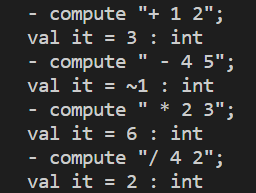
\includegraphics[width=8cm]{test2.png}
    \caption{四則演算のテスト結果}
\end{figure}




\section{課題4のプログラムの説明}
課題4では括弧を使って数式を計算できるようにした。
以下でその変更点について述べる.
\subsection{変更点}
変更点は以下の通りである.
\begin{enumerate}
    \item EXP関数で"("を取得できるようにした.
    \item COMP関数で"("と対応する")"内の処理を実行して二つの括弧を計算式の文字列から削除する.
\end{enumerate}
\subsection{変更部分のコード}
\begin{lstlisting}[caption=EXP関数の一部,label=fuga]
    fun EXP nil = raise SyntaxError
    | EXP (h::t) =
      if isInt h then (toInt h, t)
      else if h = "(" orelse h = "+" orelse h = "-" orelse h = "*" orelse h = "/" then COMP (h::t)
      else raise SyntaxError
\end{lstlisting}
\begin{lstlisting}[caption=COMPに新たに追加した分岐,label=fuga]
    if h = "(" then
    let
        val (v1,t1) = EXP t

        fun splitList lst =
            case lst of
                [] => raise SyntaxError
            | hd::tl => (hd, tl)

        val (head,t2) = splitList t1
    in
        if head = ")" then
            let
            in
                (v1, t2)
            end
        else
            raise SyntaxError
    end
\end{lstlisting}
\subsection{処理の実装}
変更点で述べた内容の詳細および実装法について述べる.
\begin{enumerate}
    \item 括弧を用いた数式の計算を実装するためにListing 3の4行目のようにEXP関数内の演算子の判定に"("を追加した.これにより,EXP関数で与えられた文字列の最初の文字が"("であるときもCOMP関数に飛ぶことができるようになった.
    また,演算子と同等の扱いにした理由は"("の中に再び"("があった際に再帰的に呼び出すことができるようにするためである.
    \item Listing 4の1行目のようにCOMP関数内の条件分岐に先頭の文字が"("である場合を追加した.この分岐内では3行目のように一度EXP関数が呼び出されてv1に先頭の文字が,t1に残りの文字列が格納される.このとき,v1が"("であった場合と演算子であった場合に処理が分岐する.
    \begin{itemize}
        \item 先頭が演算子の時\mbox{}\\
        COMP関数が呼び出されて課題3で実装した計算の処理が実行される.計算された後にv1に入るのは計算結果の数値で,t1に入るのは元の文字列から"("と,計算に使用した文字と,数字2つを取り除いた文字列が格納される.
        \item 先頭が"("のとき\mbox{}\\
        再びCOMP関数が呼び出されてその中の"("の条件分岐内でEXP関数が同じように呼び出される.
    \end{itemize}
    その後,残りの文字列の
    先頭を確かめるために5から8行目のように関数splitListを定義している.そして10行目でsplitListを使用してt1をheadとt2に分解している.
    正しく数式が入力されていればheadには")"が入力されているはずであるので12行目のように判定して一致していればv1とt2を返し,一致してなければSyntaxErrorを返す.
    再帰的に呼び出された際も"("と")"をセットで処理を行うので対応関係は守られる.
\end{enumerate}

\subsection{テスト結果}
以下の図2の一つ目のように括弧を含めた数式の計算ができるようになり,二つ目の実行例のように括弧の対応関係が取れていない数式に対してはSyntaxErrorを返すことができるようになった.
\begin{figure}[h]
    \centering
    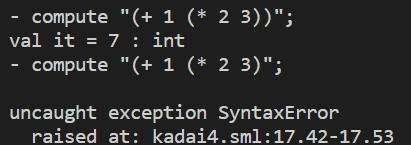
\includegraphics[width=8cm]{test3.png}
    \caption{課題4のテスト結果}
\end{figure}
\section{課題5のプログラムの説明}

課題5では"fibo"と"fact"という計算するための関数を使えるようにした.
\subsection{変更点}
変更点は以下の通りである.\\
\begin{enumerate}
    \item 新たに関数FUNCを定義し,その中に"括弧の処理とfact"と"fibo"の処理を記述した.
    \item EXP関数で先頭の文字だけでなく二文字目も取り出して"("の次の文字も判定するようにした.
\end{enumerate}

\subsection{処理の実装}
変更点で述べた内容の詳細および実装法について述べる.
\begin{enumerate}
    \item 先頭の文字が"("か"fact"か"fibo"で条件を分岐させる."("内の処理は課題4のときの処理と同じである.また,これまでとは違い,数式の文字列を先頭の文字であるhと先頭から二番目の文字であるh1とそれら以外残りの文字列であるtに分けている.
    \begin{lstlisting}[caption = EXP関数の一部,label = fuga]
        if isInt h then (toInt h, [h1]@t)
            else if h = "(" then
                if h1 = "+" orelse h1 = "-" orelse h1 = "*" orelse h1 = "/" then COMP (h::[h1]@t)
                else if isAlp h1 then FUNC (h::[h1]@t)
                else raise SyntaxError
            else if h = "+" orelse h = "-" orelse h = "*" orelse h = "/" then COMP (h::[h1]@t)
            else if isAlp h then FUNC (h::[h1]@t)
    \end{lstlisting}
    また,ここで"("の条件分岐を考えている理由としては,上のListing5のEXP関数のFUNCに飛ぶ際の処理でhが"("と一致すればさらに次の要素であるh1がアルファベットであったときに
    "("から始まる文字列を渡しているためである.ここではh1とtを連結した文字列がそれに対応する."("から渡していないと,その"("に対応する")"が出てきたときにエラーが起きてしまうためである.また,"fibo"と"fact"はlib.smlで実装されていたのでそのまま使用した.
    \item これまでは"("と演算子の分岐を同時に行っていたが,新たな関数FUNCに分岐させるために"("はほかの演算子たちとの分岐とは独立させ,またその中にさらに次の要素が何であるかを判定する分岐を作成した.具体的には次の要素が演算子であるか
    アルファベットであるかという条件分岐を作成した.演算子であればCOMPを呼び出し,アルファベットであればFUNCを呼び出して処理を行う.
\end{enumerate}

\subsection{テスト結果}
以下の図3のようにfiboやfactを含めた数式の計算を実行できるようになった.
\begin{figure}[h]
    \centering
    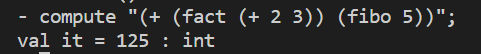
\includegraphics[width=8cm]{test4.png}
    \caption{テスト結果}
\end{figure}
\section{課題6のプログラムの説明}
課題6では数式文字列以外の引数として変数マッピングリストをとるようにし,数式中に登場した変数名に対応する数値をそのリストから取り出して置き換えることができるようにした.
\subsection{変更点}
具体的なコードの変更点は以下の通りである.
\begin{enumerate}
    \item 関数computeに二つ目の引数mapLの追加.
    \item 注目している文字がマッピングリストに存在すれば対応する数値を取り出して返す関数findValueの実装.
\end{enumerate}
\subsection{処理の実装}
変更点で述べた内容の詳細および実装法について述べる.
\begin{enumerate}
    \item 関数computeが文字列sだけでなく(string * int)型の要素を持つリストであるmapLも引数に持つので,このとき型明示は変更点のコードのように行った.
    \begin{lstlisting}[caption = 型変換,label = fuga]
    fun compute (s : string) (mapL : (string * int)list) =
    \end{lstlisting}
    また,マッピングリスト内の変数名と課題5で実装した"fact"と"fibo"を
    区別するために先に先頭の文字が"fibo"と"fact"のいずれかであるかを判定してその後にアルファベットであるかどうかの判定を行った.
    \begin{lstlisting}[caption = EXP関数の一部,label = fuga]
        fun EXP nil = raise SyntaxError
          | EXP (h::h1::t) =
            if isInt h then (toInt h, [h1]@t)
            else if h = "(" then 
                if h1 = "+" orelse h1 = "-" orelse h1 = "*" orelse h1 = "/" then COMP (h::[h1]@t)
                else if isAlp h1 then FUNC (h::[h1]@t)
                else raise SyntaxError
            else if h = "+" orelse h = "-" orelse h = "*" orelse h = "/" then COMP (h::[h1]@t)
            else if h = "fact" orelse h = "fibo" then FUNC (h::[h1]@t)
            else if isAlp h then (findValue h mapL,[h1]@t) 
            else raise SyntaxError

    \end{lstlisting}
        先頭の文字が"fibo"と"fact"のいずれかであった場合はFUNCを呼び出して課題5で記述した通りの処理を行う.先頭の文字がアルファベットであった場合は
    findValue関数を呼び出す.このときの引数は先頭のアルファベットとmapLである.findValue内の具体的な処理は2で記述する.
    \item findValue関数では引数のアルファベットがmapLの中に存在するかをfindValue自身を再帰的に呼び出すことで判定している.リストを先頭の要素であるsとそれ以外の要素であるtに分解し,sの一つ目の要素をname,二つ目の要素をvalueと型明示している.
    nameが引数として与えられた存在するか判定したいアルファベットであるsと一致しているかどうかを判定し,一致していればvalueを返す.一致していなければsとリストの残りの要素tをfindValue関数に渡し同じように処理を行う.最後の要素まで確認してnameと一致しなければSyntaxErrorを返す.
\end{enumerate}
\subsection{テスト結果}
以下の図4のように数式中にマッピングリスト内に登場する変数を利用できるようになった.
\begin{figure}[h]
    \centering
    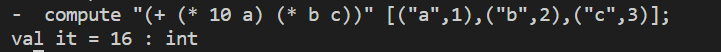
\includegraphics[width=8cm]{test5.png}
    \caption{テスト結果}
\end{figure}
\section{拡張機能の説明}
今回私は拡張機能の1番に取り組んだ.
\subsection{変更点}
COMP関数の四則演算の処理を変更した.
\subsection{処理の実装}
引き算と割り算のときに計算結果が合わなくなってしまうため,前の二つから計算を実行するようにして実現した.途中の計算の種類が変わるだけなので足し算の時の処理のみを代表的に説明する.
具体的にはCOMP関数でどの演算子なのかを取り出してから2つ先までの数値をEXP関数を2回呼び出して取り出す.そしてそれらを足し合わせてvという変数に格納しておく.そのあと
課題4の時と同様にsplitList関数を定義して3番目の要素を文字列として取り出す.その3番目の要素が数値でなければvが返り値となる.そして数値であればspllitList関数で先頭から4番目の文字を取り出して
3番目の要素を数値に変換する.4番目の要素が数値でなければvに3番目の要素を足したものが返り値となり,数値であれば演算子,vの値,3番目の要素を含めたそれ以降の文字列を結合しCOMPを再帰的に呼び出す.
\subsection{テスト結果}
以下の図のように数式中に数値だけが登場するのであれば正しく計算することができた.
\begin{figure}[h]
    \centering
    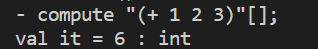
\includegraphics[width=8cm]{kakutyou.png}
    \caption{拡張課題のテスト結果}
\end{figure}
\section{今回の課題に対する考察}
拡張課題1において変数が数式の最後の方に登場してしまうとエラーが発生してしまった.これの原因としては,
"+ 1 2 3"のように連続した計算で数式が終了する場合の処理で4つ先までEXP関数を使わずに読んでしまうためfindValueが呼び出されない事が考えられる.
ただ,この4つ先まで読むという処理を実装した理由としてはcompute関数において数式を先頭,二番目,残りの三つに分けたことで残りの部分に何も入らなくなるとエラーが発生してしまったからである.
なので数式を先頭と残りに分け,課題4のif文のlet環境内で次の文字をsplitList関数を使って実装

\end{document}